\documentclass[../report.tex]{subfiles}
\begin{document}
    
    \begin{frame}
        \frametitle{4b: Viola Jones Features}
        \begin{figure}[!htb]
            \centering
            \frame{
\includegraphics[keepaspectratio,height=0.65\textheight,width=0.45\textwidth]{ps6-4-b-1}}
            \caption{ps6-4-b-1}
        \end{figure}
    \end{frame}

    \begin{frame}
        \frametitle{4b: Viola Jones Features}
        \begin{figure}[!htb]
            \centering
            \frame{
\includegraphics[keepaspectratio,height=0.65\textheight,width=0.45\textwidth]{ps6-4-b-2}}
            \caption{ps6-4-b-2}
        \end{figure}
    \end{frame}

    \begin{frame}[t]
        \frametitle{4b: Analysis}
        \begin{normalsize}
            \begin{itemize}
                \setlength\itemsep{1em}\fontsize{6pt}{6pt}

                \item[]{\textbf{\selectfont\textcolor{blue}{ Report the classifier accuracy both the training and test sets with a number of classifiers set to 5. What do the selected Haar features mean? How do they contribute in identifying faces in an image? }}}
                
                \item[]\textbf{The results from the classifier is the following:\\
Prediction accuracy on training: 98.57\\
Prediction accuracy on testing: 45.71\\
The selected Haar Features are the features that will be used\\
in the evaluation of whether or not an image is a face.\\

}
            \end{itemize}
        \end{normalsize}
    \end{frame}

    \begin{frame}
        \frametitle{4c: Viola Jones Face Recognition}
        \begin{figure}[!htb]
            \centering
            \frame{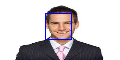
\includegraphics[keepaspectratio,height=0.65\textheight,width=0.45\textwidth]{ps6-4-c-1}}
            \caption{ps6-4-c-1}
        \end{figure}
    \end{frame}
    
\end{document}